
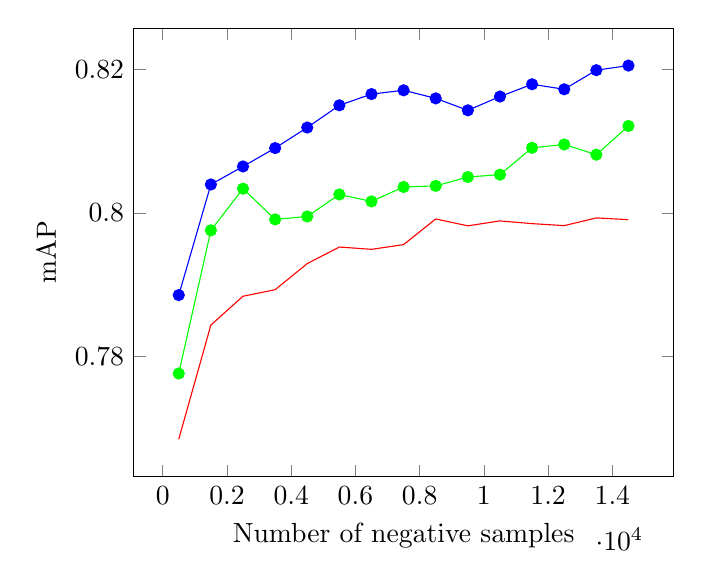
\begin{tikzpicture}
	\begin{axis}[
		xlabel=Number of negative samples,
		ylabel=mAP]
%% Poly SLEM
	\addplot[color=blue,mark=*] coordinates {
		(500,  0.78852)
		(1500, 0.80397)
		(2500, 0.80648)
		(3500, 0.80905)
		(4500, 0.81192)
		(5500, 0.81502)
		(6500, 0.81659)
		(7500, 0.81712)
		(8500, 0.81599)
		(9500, 0.81432)
		(10500,0.81625)
		(11500,0.81796)
		(12500,0.81726)
		(13500,0.81993)
		(14500,0.82057)
	};

%% Gaussian SLEM
	\addplot[color=green,mark=*] coordinates {
		(500,  0.77757)
		(1500, 0.79756)
		(2500, 0.80338)
		(3500, 0.79909)
		(4500, 0.79950)
		(5500, 0.80257)
		(6500, 0.8016)
		(7500, 0.80362)
		(8500, 0.80377)
		(9500, 0.80501)
		(10500,0.80534)
		(11500,0.80909)
		(12500,0.80955)
		(13500,0.80813)
		(14500,0.81214)
	};
%% ESVM
	\addplot[color=red] coordinates {
		(500,  0.7684)
		(1500, 0.78434)
		(2500, 0.78836)
		(3500, 0.78927)
		(4500, 0.79292)
		(5500, 0.79523)
		(6500, 0.79491)
		(7500, 0.79557)
		(8500, 0.79915)
		(9500, 0.79819)
		(10500,0.79888)
		(11500,0.7985)
		(12500,0.79822)
		(13500,0.79930)
		(14500,0.79905)
	};
	\end{axis}
\end{tikzpicture}

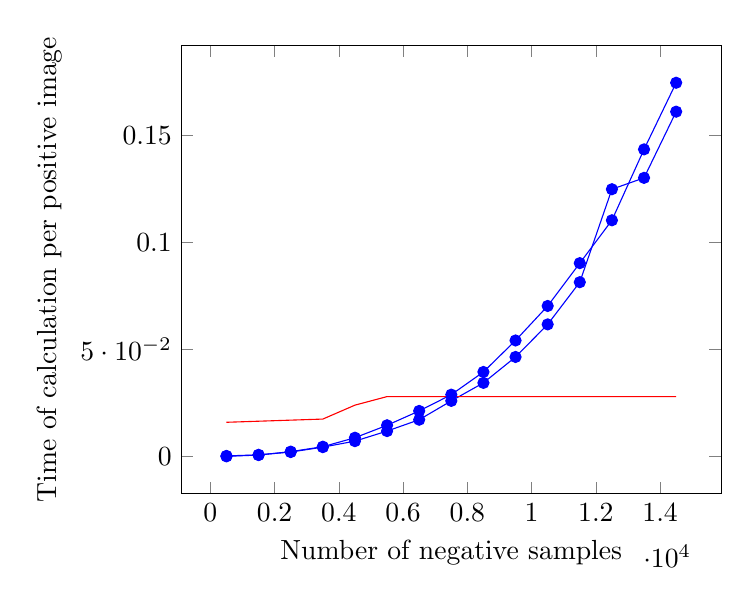
\begin{tikzpicture}
	\begin{axis}[
		xlabel=Number of negative samples,
		ylabel=Time of calculation per positive image]
%% Poly SLEM
	\addplot[color=blue,mark=*] coordinates {
		(500,  0.0001)
		(1500, 0.0007)
		(2500, 0.0023)
		(3500, 0.0046)
		(4500, 0.0088)
		(5500, 0.0146)
		(6500, 0.0213)
		(7500, 0.0289)
		(8500, 0.0395)
		(9500, 0.0542)
		(10500,0.0703)
		(11500,0.0903)
		(12500,0.1103)
		(13500,0.1434)
		(14500,0.1745)
	};
%% Gaussian SLEM
	\addplot[color=blue,mark=*] coordinates {
		(500,  0.0003)
		(1500, 0.0008)
		(2500, 0.0021)
		(3500, 0.0044)
		(4500, 0.0072)
		(5500, 0.0119)
		(6500, 0.0172)
		(7500, 0.026)
		(8500, 0.0344)
		(9500, 0.0465)
		(10500,0.0617)
		(11500,0.0814)
		(12500,0.1248)
		(13500,0.1301)
		(14500,0.161)
	};
%% ESVM
	\addplot[color=red] coordinates {
		(500,  0.016)
		(1500, 0.0165)
		(2500, 0.017)
		(3500, 0.0175)
		(4500, 0.024)
		(5500, 0.028)
		(6500, 0.028)
		(7500, 0.028)
		(8500, 0.028)
		(9500, 0.028)
		(10500,0.028)
		(11500,0.028)
		(12500,0.028)
		(13500,0.028)
		(14500,0.028)
	};
	\end{axis}
\end{tikzpicture}

